The implementation of LM includes a compiler and a virtual machine that runs
byte-code. The virtual machine uses 32 registers for
operations and executes procedures to iterate over the database in order to match facts.

\subsection{Compilation}

The compiler translates each rule to a procedure and a list of facts that need
to exist to satisfy the rule. This procedure is executed by the virtual
machine whenever we have enough facts to satisfy the rule. The procedure
loops over all possible combinations of the rule, retrieving facts from the
database, performing join operations and then consuming and deriving facts.

Optimizations such as join optimizations (to allow rule filtering invalid
combinations) and fact updates are implemented by the compiler. The latter
transforms fact derivations of the same predicate to a simple update operation,
avoiding a deallocation operation followed by an allocation of the new fact.

\subsection{Node partitioning}

The compiler builds a representation of the graph by inspecting axioms of the
program. Next, it orders the nodes of the graph using a breadth-first
topological sort. This node ordering is written to the byte-code file and then
used to initially partition nodes across available threads.

\subsubsection{Coordination directives}

Coordination directives are compiled in two different ways, depending whether they
appear in the body or in the head of the rule. Coordination facts in the body
are compiled into special instructions that inspect the state of the virtual
machine. For example, the directive \texttt{node-priority} will inspect the
target node, retrieve the current priority and assign the priority to a
register. Coordination facts in the head of the rule are also implemented as
special instructions of the virtual machine, but they perform some action,
instead of returning something. While these are still facts from the point of
view of the language, they are consumed immediatelly in order to apply the
operation, instead of being derived like any other regular fact. This is more
efficient since we do not need to create a new fact.

\subsection{Execution}

The virtual machine is implemented in C++11 and uses the threading system from
the standard library to implement multithreading. Each thread is responsible
for executing a subset of nodes. Nodes are either inactive, with no new facts,
or active, where they will be placed in the corresponding thread's queue.
Threads do useful work by processing the nodes in their queues. Whenever a
thread becomes idle, it attempts to steal nodes from a random thread into its
own queues. If unsuccessful, the thread synchronizes with the other threads to
become inactive.

\subsubsection{Nodes}

A node is represented as a collection of facts (per predicate) and an indexing structure that
keeps track of the available predicates and potential candidate rules. We need
a separate indexing structure per node since rules run locally.

Facts need to be stored efficiently because the virtual machine instructions
perform searches on the database by fixing arguments of a predicate to concrete
values. Each predicate is stored using one of the following data structures:

\begin{itemize}
\item \emph{Tries} are used exclusively to store 
  persistent facts. Tries are trees where facts are indexed by common
  prefix arguments.
\item \emph{Doubly Linked Lists} are used to store 
  linear facts. We use a double linked list because it is a very
   efficient way to add and remove facts.
\item \emph{Hash Tables} are used to improve lookup when 
  linked lists are too long and when we need to do search filtered by
  a fixed argument. The virtual machine decides which arguments are
  best to be indexed and then uses a hash table
  indexed by the appropriate argument.
\end{itemize}

A node goes through different states during execution. The state machine in
Fig.~\ref{fig:node_states} represents the valid state transitions with the
following states:

\begin{description}
   \item[working]: the node is being executed.
   \item[idle]: the node is not active, has no new facts and is not in any
   queue for processing.
   \item[queue]: the node is active with new facts and is waiting in some queue
   to be processed.
   \item[stealing]: the node has just been stolen is about to move to another
   thread.
   \item[coordinating]: the node is moving from one queue to another (i.e.
         changing priority).
\end{description}

\begin{figure}[h!]
   \centering
   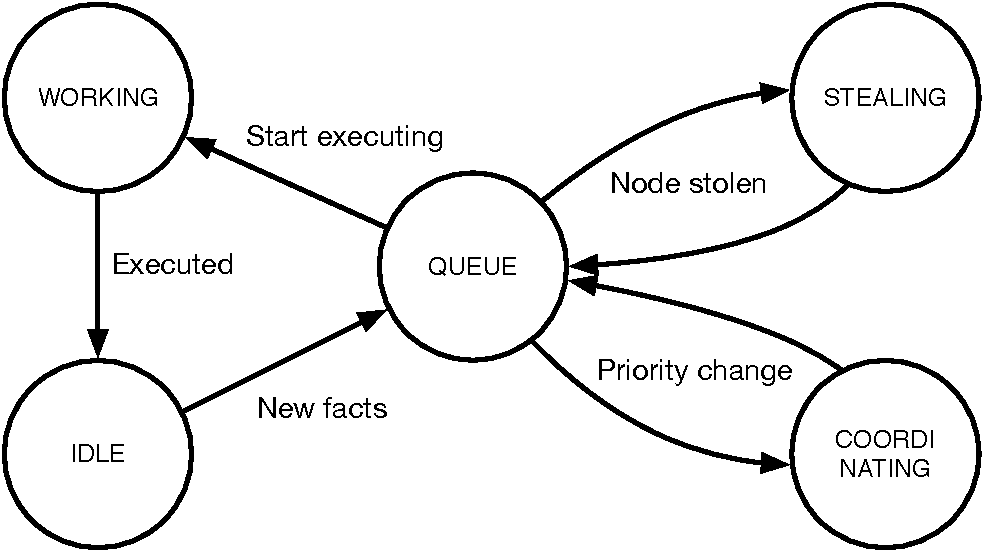
\includegraphics[width=0.4\textwidth]{node_states.pdf}
   \caption{The node state machine. During the lifetime of a program, each node
   goes through different states as specified by the state machine.}
   \label{fig:node_states}
\end{figure}

Each node is protected by a main spinlock that allows threads to change node
attributes: incoming facts, owner thread, node state and locality information.
There is also an internal spinlock that is locked whenever the node enters into
the \textbf{working} state. If a thread sends facts to a node placed in
another thread, it attempts to lock the internal lock in order to update the
indexing structures of the node, otherwise it adds the facts to the list of
incoming facts that are later processed by the owner thread.

\subsubsection{Threads}

Threads pop active nodes from their queues and execute new candidate rules. 
Each thread has 2 queues, a doubly linked list known as the \emph{standard
queue} and a min/max heap known as the \emph{priority queue}. The regular queue
contains nodes without priorities and
implements the operations \texttt{push\_tail(node)} (push to the tail),
\texttt{pop\_head()} (remove node from the head),
\texttt{remove(node)} (remove an arbitrary node) and \texttt{remove\_half()}
(removes first half). The priority queue contains nodes
with priorities and is implemented as a binary heap array. It supports the
operations \texttt{push(node,priority)} (add new node to the heap),
           \texttt{pop\_min()} (remove the best node),
\texttt{remove(node)} (remove an arbitrary node), \texttt{pop\_half\_min()}
(remove the best half) and \texttt{move(node,new\_priority)} (update priority).
Operations such as \texttt{remove\_half()} are supported in order to support
node stealing, while operations \texttt{remove(node)} or
\texttt{move(node,new\_priority)} allows threads to change the priority of
nodes.

The \texttt{next} and \texttt{prev} pointers of the regular queue are part of
the node structure in order to save space. These pointers are also used as the
index in the priority queue and current priority, respectively.

Both the regular and priority queue are actually implemented as 2 queues each.
The \emph{static queue} contains nodes that are local to a thread (and thus cannot be stolen) and
the \emph{dynamic queue} maybe accessed by other threads during node stealing.

\subsubsection{Communication}

Threads synchronize with each other using mutual exclusion. We use a spinlock in
each queue to protect queue operations and one spinlock to protect the thread's
state. Given threads $T_1$ and $T_2$, we enumerate the most important
synchronization intensive places in the virtual machine:

\begin{description}
   \item[New facts:] When a node executes on $T_1$ and derives facts
   to a node in $T_2$, $T_1$ first buffers the facts 
   and then sends them to the target node. Here, it checks if the
   node is currently \textbf{idle} and then synchronizes with $T_2$ to add the
   node to the $T_2$'s queue.
   \item[Thread activation:] If $T_2$ is inactive when adding facts to a node in
   $T_2$, $T_1$ also synchronizes with $T_2$ to change $T_2$'s state to \emph{active}.
   \item[Node stealing:] $T_1$ synchronizes with $T_2$ when it attempts to steal
   nodes from $T_2$ by removing half of the nodes from $T_2$'s queues.
   \item[Coordination:] If $T_1$ needs to perform coordination operations
   to a node in $T_2$, it may need to sychronize with $T_2$ during priority
   updates in order to move the node in $T_2$'s queues.
\end{description}

\subsubsection{Termination}

There is a global atomic counter, a global boolean flag and one boolean flag
(active/idle) per thread for detecting termination. Once a thread goes idle,
it decrements the global counter and changes its flag to idle. If the counter
goes to zero, the global flag is set to idle. Since every thread will be
busy-waiting and checking the global flag, they will detect the change and exit
the program.

\subsubsection{Node collection}

Whenever a node has an empty database and no references from other nodes, it is
deleted from the graph. The virtual machine detects such cases by keeping a
count of fact references to every node. Once the count drops to zero and the
database is empty, the node is immediatelly deleted in order to reduce memory
usage.
